\section{素材放哪里}
\label{sec:00-assets}

图片和代码按"越专用越靠近正文"放，路径\textbf{相对所在单元的目录}写。
本节用来演示的图就放在本节自己的目录里：

\begin{figure}[htbp]
\centering
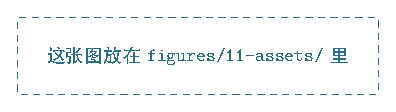
\includegraphics[width=.72\linewidth]{figures/11-assets/demo-marker}
\caption{本节专用图：放在 \texttt{figures/11-assets/} 下}
\label{fig:00-marker}
\end{figure}

\cref{fig:00-marker} 引用的是 \texttt{figures/11-assets/demo-marker}，
路径里没有出现 \texttt{chapters/} 或 \texttt{00-typesetting-guide/}——
因为章里的路径都相对本章目录。这样调整章节顺序时，素材会跟着章目录一起走。

三层规则如下。引用素材都写成 \verb|\includegraphics{路径}|，区别只在\textbf{路径怎么写}：

\begin{table}[htbp]
\centering
\caption{素材放在哪一层}
\label{tab:00-asset-levels}
\begin{tabularx}{\linewidth}{@{}P{22mm}P{54mm}Y@{}}
\toprule
通用程度 & 放在哪里 & 路径怎么写 \\
\midrule
本节专用 & 本章的 \texttt{figures/}、\texttt{code/} 下，
  按节文件名建子目录 & \texttt{figures/05-pictures/demo-flow} \\
本章多节共用 & 本章的 \texttt{figures/}、\texttt{code/} 根下 &
  \texttt{figures/chapter-overview} \\
跨章复用 & 放在主用它的那一章，别的章引用 & 从本章出发写
  \texttt{../NN-xxx/figures/文件名} \\
\bottomrule
\end{tabularx}
\end{table}

本章两种用法都有实例：\cref{fig:00-flow} 是第 5 节专用的图，放在
\texttt{figures/05-pictures/} 下；\cref{fig:00-marker} 是本节专用的图，
放在 \texttt{figures/11-assets/} 下。

还有几条规矩：

\begin{itemize}
  \item 文件名用小写英文加连字符，例如 \texttt{pipeline-hazard.pdf}，
        \textbf{不要用中文名和空格}——空格在某些工具里会出问题；
  \item 图片优先用矢量格式（PDF、SVG），位图用 PNG，照片用 JPG；
  \item 跨章复用的图只存一份，不要复制到多个章；用
        \texttt{../NN-xxx/figures/文件名} 引用；
  \item 前言和附录是全书级文件，由 \texttt{main.tex} 直接读入，
        引用素材时写从仓库根目录起的路径，例如 \texttt{backmatter/code/hello.c}；
  \item 每份素材注明来源与许可，第三方图片要确认可用范围。
\end{itemize}

\KeyPoint{路径记不住怎么办}{只记一句话：\textbf{路径相对你现在写的这个文件所在的单元目录}。
写的时候照着同一章其它地方的写法抄一遍，改文件名即可。}
